\documentclass[letterpaper,12pt]{article}
\usepackage[margin=0in]{geometry}
\usepackage[T1]{fontenc}
\usepackage{lmodern}
\pdfmapfile{+lm.map}
\pdfmapfile{+cm.map}
\usepackage{tikz}
\usetikzlibrary{arrows.meta}
\pagestyle{empty}
\setlength{\parindent}{0pt}
\hyphenpenalty=10000
\exhyphenpenalty=10000
\renewcommand{\familydefault}{\sfdefault}
\begin{document}
\begin{tikzpicture}[remember picture,overlay,x=1mm,y=1mm]
\begin{scope}[shift={(current page.north west)}]
\node[anchor=north west,inner sep=0pt,align=left,text width=180mm,font=\fontsize{11.5}{14}\selectfont\bfseries] at (18,-15.5) {Week 12 / Catalan bijections / K--1};
\node[anchor=north west,inner sep=0pt,align=left,text width=180mm,font=\fontsize{9}{11}\selectfont] at (18,-266.5) {Bellingham Math Circle / Week 12 / W12-K-v3};
\node[anchor=north east,inner sep=0pt,font=\fontsize{9}{11}\selectfont] at (198,-266.5) {1};
\node[anchor=north west,inner sep=0pt,align=left,text width=180mm,font=\fontsize{12.5}{15.5}\selectfont] at (18,-29) {Use each dot once. Keep dots in place. Strings stay inside the circle without crossings. Pairings are different when a dot has a different partner. Use strings on large circles and a pencil on small circles.};
\node[anchor=north west,inner sep=0pt,align=left,text width=180mm,font=\fontsize{12.5}{15.5}\selectfont] at (18,-51) {The two pairings of four dots:};
\draw[gray!55,line width=.45pt] (58,-84) circle (20mm);
\draw[line width=1.05pt] (58,-64) -- (78,-84);
\draw[line width=1.05pt] (58,-104) -- (38,-84);
\fill (58,-64) circle (1.45mm);
\node[inner sep=0pt,font=\fontsize{9}{10}\selectfont] at (58,-59.7) {1};
\fill (78,-84) circle (1.45mm);
\node[inner sep=0pt,font=\fontsize{9}{10}\selectfont] at (82.3,-84) {2};
\fill (58,-104) circle (1.45mm);
\node[inner sep=0pt,font=\fontsize{9}{10}\selectfont] at (58,-108.3) {3};
\fill (38,-84) circle (1.45mm);
\node[inner sep=0pt,font=\fontsize{9}{10}\selectfont] at (33.7,-84) {4};
\draw[gray!55,line width=.45pt] (159,-84) circle (20mm);
\draw[line width=1.05pt] (159,-64) -- (139,-84);
\draw[line width=1.05pt] (179,-84) -- (159,-104);
\fill (159,-64) circle (1.45mm);
\node[inner sep=0pt,font=\fontsize{9}{10}\selectfont] at (159,-59.7) {1};
\fill (179,-84) circle (1.45mm);
\node[inner sep=0pt,font=\fontsize{9}{10}\selectfont] at (183.3,-84) {2};
\fill (159,-104) circle (1.45mm);
\node[inner sep=0pt,font=\fontsize{9}{10}\selectfont] at (159,-108.3) {3};
\fill (139,-84) circle (1.45mm);
\node[inner sep=0pt,font=\fontsize{9}{10}\selectfont] at (134.7,-84) {4};
\node[anchor=north west,inner sep=0pt,align=left,text width=180mm,font=\fontsize{14}{17.5}\selectfont] at (18,-119) {\textbf{Problem 1:} Find every way to pair six dots.};
\draw[gray!55,line width=.45pt] (61,-188) circle (32mm);
\fill (61,-156) circle (1.45mm);
\node[inner sep=0pt,font=\fontsize{9}{10}\selectfont] at (61,-143.5) {1};
\fill (88.713,-172) circle (1.45mm);
\node[inner sep=0pt,font=\fontsize{9}{10}\selectfont] at (99.538,-165.75) {2};
\fill (88.713,-204) circle (1.45mm);
\node[inner sep=0pt,font=\fontsize{9}{10}\selectfont] at (99.538,-210.25) {3};
\fill (61,-220) circle (1.45mm);
\node[inner sep=0pt,font=\fontsize{9}{10}\selectfont] at (61,-232.5) {4};
\fill (33.287,-204) circle (1.45mm);
\node[inner sep=0pt,font=\fontsize{9}{10}\selectfont] at (22.462,-210.25) {5};
\fill (33.287,-172) circle (1.45mm);
\node[inner sep=0pt,font=\fontsize{9}{10}\selectfont] at (22.462,-165.75) {6};
\draw[gray!55,line width=.45pt] (131,-154) circle (15mm);
\fill (131,-139) circle (1.45mm);
\node[inner sep=0pt,font=\fontsize{9}{10}\selectfont] at (131,-134.7) {1};
\fill (143.99,-146.5) circle (1.45mm);
\node[inner sep=0pt,font=\fontsize{9}{10}\selectfont] at (147.714,-144.35) {2};
\fill (143.99,-161.5) circle (1.45mm);
\node[inner sep=0pt,font=\fontsize{9}{10}\selectfont] at (147.714,-163.65) {3};
\fill (131,-169) circle (1.45mm);
\node[inner sep=0pt,font=\fontsize{9}{10}\selectfont] at (131,-173.3) {4};
\fill (118.01,-161.5) circle (1.45mm);
\node[inner sep=0pt,font=\fontsize{9}{10}\selectfont] at (114.286,-163.65) {5};
\fill (118.01,-146.5) circle (1.45mm);
\node[inner sep=0pt,font=\fontsize{9}{10}\selectfont] at (114.286,-144.35) {6};
\draw[gray!55,line width=.45pt] (177,-154) circle (15mm);
\fill (177,-139) circle (1.45mm);
\node[inner sep=0pt,font=\fontsize{9}{10}\selectfont] at (177,-134.7) {1};
\fill (189.99,-146.5) circle (1.45mm);
\node[inner sep=0pt,font=\fontsize{9}{10}\selectfont] at (193.714,-144.35) {2};
\fill (189.99,-161.5) circle (1.45mm);
\node[inner sep=0pt,font=\fontsize{9}{10}\selectfont] at (193.714,-163.65) {3};
\fill (177,-169) circle (1.45mm);
\node[inner sep=0pt,font=\fontsize{9}{10}\selectfont] at (177,-173.3) {4};
\fill (164.01,-161.5) circle (1.45mm);
\node[inner sep=0pt,font=\fontsize{9}{10}\selectfont] at (160.286,-163.65) {5};
\fill (164.01,-146.5) circle (1.45mm);
\node[inner sep=0pt,font=\fontsize{9}{10}\selectfont] at (160.286,-144.35) {6};
\draw[gray!55,line width=.45pt] (131,-198) circle (15mm);
\fill (131,-183) circle (1.45mm);
\node[inner sep=0pt,font=\fontsize{9}{10}\selectfont] at (131,-178.7) {1};
\fill (143.99,-190.5) circle (1.45mm);
\node[inner sep=0pt,font=\fontsize{9}{10}\selectfont] at (147.714,-188.35) {2};
\fill (143.99,-205.5) circle (1.45mm);
\node[inner sep=0pt,font=\fontsize{9}{10}\selectfont] at (147.714,-207.65) {3};
\fill (131,-213) circle (1.45mm);
\node[inner sep=0pt,font=\fontsize{9}{10}\selectfont] at (131,-217.3) {4};
\fill (118.01,-205.5) circle (1.45mm);
\node[inner sep=0pt,font=\fontsize{9}{10}\selectfont] at (114.286,-207.65) {5};
\fill (118.01,-190.5) circle (1.45mm);
\node[inner sep=0pt,font=\fontsize{9}{10}\selectfont] at (114.286,-188.35) {6};
\draw[gray!55,line width=.45pt] (177,-198) circle (15mm);
\fill (177,-183) circle (1.45mm);
\node[inner sep=0pt,font=\fontsize{9}{10}\selectfont] at (177,-178.7) {1};
\fill (189.99,-190.5) circle (1.45mm);
\node[inner sep=0pt,font=\fontsize{9}{10}\selectfont] at (193.714,-188.35) {2};
\fill (189.99,-205.5) circle (1.45mm);
\node[inner sep=0pt,font=\fontsize{9}{10}\selectfont] at (193.714,-207.65) {3};
\fill (177,-213) circle (1.45mm);
\node[inner sep=0pt,font=\fontsize{9}{10}\selectfont] at (177,-217.3) {4};
\fill (164.01,-205.5) circle (1.45mm);
\node[inner sep=0pt,font=\fontsize{9}{10}\selectfont] at (160.286,-207.65) {5};
\fill (164.01,-190.5) circle (1.45mm);
\node[inner sep=0pt,font=\fontsize{9}{10}\selectfont] at (160.286,-188.35) {6};
\draw[gray!55,line width=.45pt] (131,-242) circle (15mm);
\fill (131,-227) circle (1.45mm);
\node[inner sep=0pt,font=\fontsize{9}{10}\selectfont] at (131,-222.7) {1};
\fill (143.99,-234.5) circle (1.45mm);
\node[inner sep=0pt,font=\fontsize{9}{10}\selectfont] at (147.714,-232.35) {2};
\fill (143.99,-249.5) circle (1.45mm);
\node[inner sep=0pt,font=\fontsize{9}{10}\selectfont] at (147.714,-251.65) {3};
\fill (131,-257) circle (1.45mm);
\node[inner sep=0pt,font=\fontsize{9}{10}\selectfont] at (131,-261.3) {4};
\fill (118.01,-249.5) circle (1.45mm);
\node[inner sep=0pt,font=\fontsize{9}{10}\selectfont] at (114.286,-251.65) {5};
\fill (118.01,-234.5) circle (1.45mm);
\node[inner sep=0pt,font=\fontsize{9}{10}\selectfont] at (114.286,-232.35) {6};
\draw[gray!55,line width=.45pt] (177,-242) circle (15mm);
\fill (177,-227) circle (1.45mm);
\node[inner sep=0pt,font=\fontsize{9}{10}\selectfont] at (177,-222.7) {1};
\fill (189.99,-234.5) circle (1.45mm);
\node[inner sep=0pt,font=\fontsize{9}{10}\selectfont] at (193.714,-232.35) {2};
\fill (189.99,-249.5) circle (1.45mm);
\node[inner sep=0pt,font=\fontsize{9}{10}\selectfont] at (193.714,-251.65) {3};
\fill (177,-257) circle (1.45mm);
\node[inner sep=0pt,font=\fontsize{9}{10}\selectfont] at (177,-261.3) {4};
\fill (164.01,-249.5) circle (1.45mm);
\node[inner sep=0pt,font=\fontsize{9}{10}\selectfont] at (160.286,-251.65) {5};
\fill (164.01,-234.5) circle (1.45mm);
\node[inner sep=0pt,font=\fontsize{9}{10}\selectfont] at (160.286,-232.35) {6};
\end{scope}
\end{tikzpicture}
\null
\newpage

\begin{tikzpicture}[remember picture,overlay,x=1mm,y=1mm]
\begin{scope}[shift={(current page.north west)}]
\node[anchor=north west,inner sep=0pt,align=left,text width=180mm,font=\fontsize{11.5}{14}\selectfont\bfseries] at (18,-15.5) {Week 12 / Catalan bijections / K--1};
\node[anchor=north west,inner sep=0pt,align=left,text width=180mm,font=\fontsize{9}{11}\selectfont] at (18,-266.5) {Bellingham Math Circle / Week 12 / W12-K-v3};
\node[anchor=north east,inner sep=0pt,font=\fontsize{9}{11}\selectfont] at (198,-266.5) {2};
\node[anchor=north west,inner sep=0pt,align=left,text width=180mm,font=\fontsize{14}{17.5}\selectfont] at (18,-30) {\textbf{Problem 2:} Check your six-dot collection. Show how you know that no pairing is missing.};
\draw[gray!55,line width=.45pt] (108,-107) circle (40mm);
\fill (108,-67) circle (1.45mm);
\node[inner sep=0pt,font=\fontsize{9}{10}\selectfont] at (108,-54.5) {1};
\fill (142.641,-87) circle (1.45mm);
\node[inner sep=0pt,font=\fontsize{9}{10}\selectfont] at (153.466,-80.75) {2};
\fill (142.641,-127) circle (1.45mm);
\node[inner sep=0pt,font=\fontsize{9}{10}\selectfont] at (153.466,-133.25) {3};
\fill (108,-147) circle (1.45mm);
\node[inner sep=0pt,font=\fontsize{9}{10}\selectfont] at (108,-159.5) {4};
\fill (73.359,-127) circle (1.45mm);
\node[inner sep=0pt,font=\fontsize{9}{10}\selectfont] at (62.534,-133.25) {5};
\fill (73.359,-87) circle (1.45mm);
\node[inner sep=0pt,font=\fontsize{9}{10}\selectfont] at (62.534,-80.75) {6};
\draw[gray!55,line width=.45pt] (41,-190) circle (18.5mm);
\fill (41,-171.5) circle (1.45mm);
\node[inner sep=0pt,font=\fontsize{9}{10}\selectfont] at (41,-167.2) {1};
\fill (57.021,-180.75) circle (1.45mm);
\node[inner sep=0pt,font=\fontsize{9}{10}\selectfont] at (60.745,-178.6) {2};
\fill (57.021,-199.25) circle (1.45mm);
\node[inner sep=0pt,font=\fontsize{9}{10}\selectfont] at (60.745,-201.4) {3};
\fill (41,-208.5) circle (1.45mm);
\node[inner sep=0pt,font=\fontsize{9}{10}\selectfont] at (41,-212.8) {4};
\fill (24.979,-199.25) circle (1.45mm);
\node[inner sep=0pt,font=\fontsize{9}{10}\selectfont] at (21.255,-201.4) {5};
\fill (24.979,-180.75) circle (1.45mm);
\node[inner sep=0pt,font=\fontsize{9}{10}\selectfont] at (21.255,-178.6) {6};
\draw[gray!55,line width=.45pt] (108,-190) circle (18.5mm);
\fill (108,-171.5) circle (1.45mm);
\node[inner sep=0pt,font=\fontsize{9}{10}\selectfont] at (108,-167.2) {1};
\fill (124.021,-180.75) circle (1.45mm);
\node[inner sep=0pt,font=\fontsize{9}{10}\selectfont] at (127.745,-178.6) {2};
\fill (124.021,-199.25) circle (1.45mm);
\node[inner sep=0pt,font=\fontsize{9}{10}\selectfont] at (127.745,-201.4) {3};
\fill (108,-208.5) circle (1.45mm);
\node[inner sep=0pt,font=\fontsize{9}{10}\selectfont] at (108,-212.8) {4};
\fill (91.979,-199.25) circle (1.45mm);
\node[inner sep=0pt,font=\fontsize{9}{10}\selectfont] at (88.255,-201.4) {5};
\fill (91.979,-180.75) circle (1.45mm);
\node[inner sep=0pt,font=\fontsize{9}{10}\selectfont] at (88.255,-178.6) {6};
\draw[gray!55,line width=.45pt] (175,-190) circle (18.5mm);
\fill (175,-171.5) circle (1.45mm);
\node[inner sep=0pt,font=\fontsize{9}{10}\selectfont] at (175,-167.2) {1};
\fill (191.021,-180.75) circle (1.45mm);
\node[inner sep=0pt,font=\fontsize{9}{10}\selectfont] at (194.745,-178.6) {2};
\fill (191.021,-199.25) circle (1.45mm);
\node[inner sep=0pt,font=\fontsize{9}{10}\selectfont] at (194.745,-201.4) {3};
\fill (175,-208.5) circle (1.45mm);
\node[inner sep=0pt,font=\fontsize{9}{10}\selectfont] at (175,-212.8) {4};
\fill (158.979,-199.25) circle (1.45mm);
\node[inner sep=0pt,font=\fontsize{9}{10}\selectfont] at (155.255,-201.4) {5};
\fill (158.979,-180.75) circle (1.45mm);
\node[inner sep=0pt,font=\fontsize{9}{10}\selectfont] at (155.255,-178.6) {6};
\draw[gray!55,line width=.45pt] (41,-240) circle (18.5mm);
\fill (41,-221.5) circle (1.45mm);
\node[inner sep=0pt,font=\fontsize{9}{10}\selectfont] at (41,-217.2) {1};
\fill (57.021,-230.75) circle (1.45mm);
\node[inner sep=0pt,font=\fontsize{9}{10}\selectfont] at (60.745,-228.6) {2};
\fill (57.021,-249.25) circle (1.45mm);
\node[inner sep=0pt,font=\fontsize{9}{10}\selectfont] at (60.745,-251.4) {3};
\fill (41,-258.5) circle (1.45mm);
\node[inner sep=0pt,font=\fontsize{9}{10}\selectfont] at (41,-262.8) {4};
\fill (24.979,-249.25) circle (1.45mm);
\node[inner sep=0pt,font=\fontsize{9}{10}\selectfont] at (21.255,-251.4) {5};
\fill (24.979,-230.75) circle (1.45mm);
\node[inner sep=0pt,font=\fontsize{9}{10}\selectfont] at (21.255,-228.6) {6};
\draw[gray!55,line width=.45pt] (108,-240) circle (18.5mm);
\fill (108,-221.5) circle (1.45mm);
\node[inner sep=0pt,font=\fontsize{9}{10}\selectfont] at (108,-217.2) {1};
\fill (124.021,-230.75) circle (1.45mm);
\node[inner sep=0pt,font=\fontsize{9}{10}\selectfont] at (127.745,-228.6) {2};
\fill (124.021,-249.25) circle (1.45mm);
\node[inner sep=0pt,font=\fontsize{9}{10}\selectfont] at (127.745,-251.4) {3};
\fill (108,-258.5) circle (1.45mm);
\node[inner sep=0pt,font=\fontsize{9}{10}\selectfont] at (108,-262.8) {4};
\fill (91.979,-249.25) circle (1.45mm);
\node[inner sep=0pt,font=\fontsize{9}{10}\selectfont] at (88.255,-251.4) {5};
\fill (91.979,-230.75) circle (1.45mm);
\node[inner sep=0pt,font=\fontsize{9}{10}\selectfont] at (88.255,-228.6) {6};
\draw[gray!55,line width=.45pt] (175,-240) circle (18.5mm);
\fill (175,-221.5) circle (1.45mm);
\node[inner sep=0pt,font=\fontsize{9}{10}\selectfont] at (175,-217.2) {1};
\fill (191.021,-230.75) circle (1.45mm);
\node[inner sep=0pt,font=\fontsize{9}{10}\selectfont] at (194.745,-228.6) {2};
\fill (191.021,-249.25) circle (1.45mm);
\node[inner sep=0pt,font=\fontsize{9}{10}\selectfont] at (194.745,-251.4) {3};
\fill (175,-258.5) circle (1.45mm);
\node[inner sep=0pt,font=\fontsize{9}{10}\selectfont] at (175,-262.8) {4};
\fill (158.979,-249.25) circle (1.45mm);
\node[inner sep=0pt,font=\fontsize{9}{10}\selectfont] at (155.255,-251.4) {5};
\fill (158.979,-230.75) circle (1.45mm);
\node[inner sep=0pt,font=\fontsize{9}{10}\selectfont] at (155.255,-228.6) {6};
\end{scope}
\end{tikzpicture}
\null
\newpage
\begin{tikzpicture}[remember picture,overlay,x=1mm,y=1mm]
\begin{scope}[shift={(current page.north west)}]
\node[anchor=north west,inner sep=0pt,align=left,text width=180mm,font=\fontsize{11.5}{14}\selectfont\bfseries] at (18,-15.5) {Week 12 / Catalan bijections / K--1};
\node[anchor=north west,inner sep=0pt,align=left,text width=180mm,font=\fontsize{9}{11}\selectfont] at (18,-266.5) {Bellingham Math Circle / Week 12 / W12-K-v3};
\node[anchor=north east,inner sep=0pt,font=\fontsize{9}{11}\selectfont] at (198,-266.5) {3};
\node[anchor=north west,inner sep=0pt,align=left,text width=180mm,font=\fontsize{13.5}{17}\selectfont] at (18,-30) {\textbf{Problem 3:} Keep each drawn pair when you try it on the large circle. Find every way to finish it, or show why you cannot.};
\draw[gray!55,line width=.45pt] (108,-107) circle (40mm);
\fill (108,-67) circle (1.45mm);
\node[inner sep=0pt,font=\fontsize{9}{10}\selectfont] at (108,-54.5) {1};
\fill (136.284,-78.716) circle (1.45mm);
\node[inner sep=0pt,font=\fontsize{9}{10}\selectfont] at (145.123,-69.877) {2};
\fill (148,-107) circle (1.45mm);
\node[inner sep=0pt,font=\fontsize{9}{10}\selectfont] at (160.5,-107) {3};
\fill (136.284,-135.284) circle (1.45mm);
\node[inner sep=0pt,font=\fontsize{9}{10}\selectfont] at (145.123,-144.123) {4};
\fill (108,-147) circle (1.45mm);
\node[inner sep=0pt,font=\fontsize{9}{10}\selectfont] at (108,-159.5) {5};
\fill (79.716,-135.284) circle (1.45mm);
\node[inner sep=0pt,font=\fontsize{9}{10}\selectfont] at (70.877,-144.123) {6};
\fill (68,-107) circle (1.45mm);
\node[inner sep=0pt,font=\fontsize{9}{10}\selectfont] at (55.5,-107) {7};
\fill (79.716,-78.716) circle (1.45mm);
\node[inner sep=0pt,font=\fontsize{9}{10}\selectfont] at (70.877,-69.877) {8};
\draw[gray!55,line width=.45pt] (41,-190) circle (18.5mm);
\draw[line width=1.05pt] (41,-171.5) -- (54.081,-203.081);
\fill (41,-171.5) circle (1.45mm);
\node[inner sep=0pt,font=\fontsize{9}{10}\selectfont] at (41,-167.2) {1};
\fill (54.081,-176.919) circle (1.45mm);
\node[inner sep=0pt,font=\fontsize{9}{10}\selectfont] at (57.122,-173.878) {2};
\fill (59.5,-190) circle (1.45mm);
\node[inner sep=0pt,font=\fontsize{9}{10}\selectfont] at (63.8,-190) {3};
\fill (54.081,-203.081) circle (1.45mm);
\node[inner sep=0pt,font=\fontsize{9}{10}\selectfont] at (57.122,-206.122) {4};
\fill (41,-208.5) circle (1.45mm);
\node[inner sep=0pt,font=\fontsize{9}{10}\selectfont] at (41,-212.8) {5};
\fill (27.919,-203.081) circle (1.45mm);
\node[inner sep=0pt,font=\fontsize{9}{10}\selectfont] at (24.878,-206.122) {6};
\fill (22.5,-190) circle (1.45mm);
\node[inner sep=0pt,font=\fontsize{9}{10}\selectfont] at (18.2,-190) {7};
\fill (27.919,-176.919) circle (1.45mm);
\node[inner sep=0pt,font=\fontsize{9}{10}\selectfont] at (24.878,-173.878) {8};
\draw[gray!55,line width=.45pt] (108,-190) circle (18.5mm);
\draw[line width=1.05pt] (108,-171.5) -- (121.081,-203.081);
\fill (108,-171.5) circle (1.45mm);
\node[inner sep=0pt,font=\fontsize{9}{10}\selectfont] at (108,-167.2) {1};
\fill (121.081,-176.919) circle (1.45mm);
\node[inner sep=0pt,font=\fontsize{9}{10}\selectfont] at (124.122,-173.878) {2};
\fill (126.5,-190) circle (1.45mm);
\node[inner sep=0pt,font=\fontsize{9}{10}\selectfont] at (130.8,-190) {3};
\fill (121.081,-203.081) circle (1.45mm);
\node[inner sep=0pt,font=\fontsize{9}{10}\selectfont] at (124.122,-206.122) {4};
\fill (108,-208.5) circle (1.45mm);
\node[inner sep=0pt,font=\fontsize{9}{10}\selectfont] at (108,-212.8) {5};
\fill (94.919,-203.081) circle (1.45mm);
\node[inner sep=0pt,font=\fontsize{9}{10}\selectfont] at (91.878,-206.122) {6};
\fill (89.5,-190) circle (1.45mm);
\node[inner sep=0pt,font=\fontsize{9}{10}\selectfont] at (85.2,-190) {7};
\fill (94.919,-176.919) circle (1.45mm);
\node[inner sep=0pt,font=\fontsize{9}{10}\selectfont] at (91.878,-173.878) {8};
\draw[gray!55,line width=.45pt] (175,-190) circle (18.5mm);
\draw[line width=1.05pt] (175,-171.5) -- (161.919,-203.081);
\fill (175,-171.5) circle (1.45mm);
\node[inner sep=0pt,font=\fontsize{9}{10}\selectfont] at (175,-167.2) {1};
\fill (188.081,-176.919) circle (1.45mm);
\node[inner sep=0pt,font=\fontsize{9}{10}\selectfont] at (191.122,-173.878) {2};
\fill (193.5,-190) circle (1.45mm);
\node[inner sep=0pt,font=\fontsize{9}{10}\selectfont] at (197.8,-190) {3};
\fill (188.081,-203.081) circle (1.45mm);
\node[inner sep=0pt,font=\fontsize{9}{10}\selectfont] at (191.122,-206.122) {4};
\fill (175,-208.5) circle (1.45mm);
\node[inner sep=0pt,font=\fontsize{9}{10}\selectfont] at (175,-212.8) {5};
\fill (161.919,-203.081) circle (1.45mm);
\node[inner sep=0pt,font=\fontsize{9}{10}\selectfont] at (158.878,-206.122) {6};
\fill (156.5,-190) circle (1.45mm);
\node[inner sep=0pt,font=\fontsize{9}{10}\selectfont] at (152.2,-190) {7};
\fill (161.919,-176.919) circle (1.45mm);
\node[inner sep=0pt,font=\fontsize{9}{10}\selectfont] at (158.878,-173.878) {8};
\draw[gray!55,line width=.45pt] (41,-240) circle (18.5mm);
\draw[line width=1.05pt] (41,-221.5) -- (27.919,-253.081);
\fill (41,-221.5) circle (1.45mm);
\node[inner sep=0pt,font=\fontsize{9}{10}\selectfont] at (41,-217.2) {1};
\fill (54.081,-226.919) circle (1.45mm);
\node[inner sep=0pt,font=\fontsize{9}{10}\selectfont] at (57.122,-223.878) {2};
\fill (59.5,-240) circle (1.45mm);
\node[inner sep=0pt,font=\fontsize{9}{10}\selectfont] at (63.8,-240) {3};
\fill (54.081,-253.081) circle (1.45mm);
\node[inner sep=0pt,font=\fontsize{9}{10}\selectfont] at (57.122,-256.122) {4};
\fill (41,-258.5) circle (1.45mm);
\node[inner sep=0pt,font=\fontsize{9}{10}\selectfont] at (41,-262.8) {5};
\fill (27.919,-253.081) circle (1.45mm);
\node[inner sep=0pt,font=\fontsize{9}{10}\selectfont] at (24.878,-256.122) {6};
\fill (22.5,-240) circle (1.45mm);
\node[inner sep=0pt,font=\fontsize{9}{10}\selectfont] at (18.2,-240) {7};
\fill (27.919,-226.919) circle (1.45mm);
\node[inner sep=0pt,font=\fontsize{9}{10}\selectfont] at (24.878,-223.878) {8};
\draw[gray!55,line width=.45pt] (108,-240) circle (18.5mm);
\draw[line width=1.05pt] (108,-221.5) -- (126.5,-240);
\fill (108,-221.5) circle (1.45mm);
\node[inner sep=0pt,font=\fontsize{9}{10}\selectfont] at (108,-217.2) {1};
\fill (121.081,-226.919) circle (1.45mm);
\node[inner sep=0pt,font=\fontsize{9}{10}\selectfont] at (124.122,-223.878) {2};
\fill (126.5,-240) circle (1.45mm);
\node[inner sep=0pt,font=\fontsize{9}{10}\selectfont] at (130.8,-240) {3};
\fill (121.081,-253.081) circle (1.45mm);
\node[inner sep=0pt,font=\fontsize{9}{10}\selectfont] at (124.122,-256.122) {4};
\fill (108,-258.5) circle (1.45mm);
\node[inner sep=0pt,font=\fontsize{9}{10}\selectfont] at (108,-262.8) {5};
\fill (94.919,-253.081) circle (1.45mm);
\node[inner sep=0pt,font=\fontsize{9}{10}\selectfont] at (91.878,-256.122) {6};
\fill (89.5,-240) circle (1.45mm);
\node[inner sep=0pt,font=\fontsize{9}{10}\selectfont] at (85.2,-240) {7};
\fill (94.919,-226.919) circle (1.45mm);
\node[inner sep=0pt,font=\fontsize{9}{10}\selectfont] at (91.878,-223.878) {8};
\draw[gray!55,line width=.45pt] (175,-240) circle (18.5mm);
\draw[line width=1.05pt] (175,-221.5) -- (175,-258.5);
\fill (175,-221.5) circle (1.45mm);
\node[inner sep=0pt,font=\fontsize{9}{10}\selectfont] at (175,-217.2) {1};
\fill (188.081,-226.919) circle (1.45mm);
\node[inner sep=0pt,font=\fontsize{9}{10}\selectfont] at (191.122,-223.878) {2};
\fill (193.5,-240) circle (1.45mm);
\node[inner sep=0pt,font=\fontsize{9}{10}\selectfont] at (197.8,-240) {3};
\fill (188.081,-253.081) circle (1.45mm);
\node[inner sep=0pt,font=\fontsize{9}{10}\selectfont] at (191.122,-256.122) {4};
\fill (175,-258.5) circle (1.45mm);
\node[inner sep=0pt,font=\fontsize{9}{10}\selectfont] at (175,-262.8) {5};
\fill (161.919,-253.081) circle (1.45mm);
\node[inner sep=0pt,font=\fontsize{9}{10}\selectfont] at (158.878,-256.122) {6};
\fill (156.5,-240) circle (1.45mm);
\node[inner sep=0pt,font=\fontsize{9}{10}\selectfont] at (152.2,-240) {7};
\fill (161.919,-226.919) circle (1.45mm);
\node[inner sep=0pt,font=\fontsize{9}{10}\selectfont] at (158.878,-223.878) {8};
\end{scope}
\end{tikzpicture}
\null
\newpage
\begin{tikzpicture}[remember picture,overlay,x=1mm,y=1mm]
\begin{scope}[shift={(current page.north west)}]
\node[anchor=north west,inner sep=0pt,align=left,text width=180mm,font=\fontsize{11.5}{14}\selectfont\bfseries] at (18,-15.5) {Week 12 / Catalan bijections / K--1};
\node[anchor=north west,inner sep=0pt,align=left,text width=180mm,font=\fontsize{9}{11}\selectfont] at (18,-266.5) {Bellingham Math Circle / Week 12 / W12-K-v3};
\node[anchor=north east,inner sep=0pt,font=\fontsize{9}{11}\selectfont] at (198,-266.5) {4};
\node[anchor=north west,inner sep=0pt,align=left,text width=180mm,font=\fontsize{14}{17.5}\selectfont] at (18,-30) {\textbf{Problem 4:} Pair eight dots in as many different ways as you can. Draw extra circles on blank paper if you need them.};
\draw[gray!55,line width=.45pt] (108,-107) circle (40mm);
\fill (108,-67) circle (1.45mm);
\node[inner sep=0pt,font=\fontsize{9}{10}\selectfont] at (108,-54.5) {1};
\fill (136.284,-78.716) circle (1.45mm);
\node[inner sep=0pt,font=\fontsize{9}{10}\selectfont] at (145.123,-69.877) {2};
\fill (148,-107) circle (1.45mm);
\node[inner sep=0pt,font=\fontsize{9}{10}\selectfont] at (160.5,-107) {3};
\fill (136.284,-135.284) circle (1.45mm);
\node[inner sep=0pt,font=\fontsize{9}{10}\selectfont] at (145.123,-144.123) {4};
\fill (108,-147) circle (1.45mm);
\node[inner sep=0pt,font=\fontsize{9}{10}\selectfont] at (108,-159.5) {5};
\fill (79.716,-135.284) circle (1.45mm);
\node[inner sep=0pt,font=\fontsize{9}{10}\selectfont] at (70.877,-144.123) {6};
\fill (68,-107) circle (1.45mm);
\node[inner sep=0pt,font=\fontsize{9}{10}\selectfont] at (55.5,-107) {7};
\fill (79.716,-78.716) circle (1.45mm);
\node[inner sep=0pt,font=\fontsize{9}{10}\selectfont] at (70.877,-69.877) {8};
\draw[gray!55,line width=.45pt] (41,-190) circle (18.5mm);
\fill (41,-171.5) circle (1.45mm);
\node[inner sep=0pt,font=\fontsize{9}{10}\selectfont] at (41,-167.2) {1};
\fill (54.081,-176.919) circle (1.45mm);
\node[inner sep=0pt,font=\fontsize{9}{10}\selectfont] at (57.122,-173.878) {2};
\fill (59.5,-190) circle (1.45mm);
\node[inner sep=0pt,font=\fontsize{9}{10}\selectfont] at (63.8,-190) {3};
\fill (54.081,-203.081) circle (1.45mm);
\node[inner sep=0pt,font=\fontsize{9}{10}\selectfont] at (57.122,-206.122) {4};
\fill (41,-208.5) circle (1.45mm);
\node[inner sep=0pt,font=\fontsize{9}{10}\selectfont] at (41,-212.8) {5};
\fill (27.919,-203.081) circle (1.45mm);
\node[inner sep=0pt,font=\fontsize{9}{10}\selectfont] at (24.878,-206.122) {6};
\fill (22.5,-190) circle (1.45mm);
\node[inner sep=0pt,font=\fontsize{9}{10}\selectfont] at (18.2,-190) {7};
\fill (27.919,-176.919) circle (1.45mm);
\node[inner sep=0pt,font=\fontsize{9}{10}\selectfont] at (24.878,-173.878) {8};
\draw[gray!55,line width=.45pt] (108,-190) circle (18.5mm);
\fill (108,-171.5) circle (1.45mm);
\node[inner sep=0pt,font=\fontsize{9}{10}\selectfont] at (108,-167.2) {1};
\fill (121.081,-176.919) circle (1.45mm);
\node[inner sep=0pt,font=\fontsize{9}{10}\selectfont] at (124.122,-173.878) {2};
\fill (126.5,-190) circle (1.45mm);
\node[inner sep=0pt,font=\fontsize{9}{10}\selectfont] at (130.8,-190) {3};
\fill (121.081,-203.081) circle (1.45mm);
\node[inner sep=0pt,font=\fontsize{9}{10}\selectfont] at (124.122,-206.122) {4};
\fill (108,-208.5) circle (1.45mm);
\node[inner sep=0pt,font=\fontsize{9}{10}\selectfont] at (108,-212.8) {5};
\fill (94.919,-203.081) circle (1.45mm);
\node[inner sep=0pt,font=\fontsize{9}{10}\selectfont] at (91.878,-206.122) {6};
\fill (89.5,-190) circle (1.45mm);
\node[inner sep=0pt,font=\fontsize{9}{10}\selectfont] at (85.2,-190) {7};
\fill (94.919,-176.919) circle (1.45mm);
\node[inner sep=0pt,font=\fontsize{9}{10}\selectfont] at (91.878,-173.878) {8};
\draw[gray!55,line width=.45pt] (175,-190) circle (18.5mm);
\fill (175,-171.5) circle (1.45mm);
\node[inner sep=0pt,font=\fontsize{9}{10}\selectfont] at (175,-167.2) {1};
\fill (188.081,-176.919) circle (1.45mm);
\node[inner sep=0pt,font=\fontsize{9}{10}\selectfont] at (191.122,-173.878) {2};
\fill (193.5,-190) circle (1.45mm);
\node[inner sep=0pt,font=\fontsize{9}{10}\selectfont] at (197.8,-190) {3};
\fill (188.081,-203.081) circle (1.45mm);
\node[inner sep=0pt,font=\fontsize{9}{10}\selectfont] at (191.122,-206.122) {4};
\fill (175,-208.5) circle (1.45mm);
\node[inner sep=0pt,font=\fontsize{9}{10}\selectfont] at (175,-212.8) {5};
\fill (161.919,-203.081) circle (1.45mm);
\node[inner sep=0pt,font=\fontsize{9}{10}\selectfont] at (158.878,-206.122) {6};
\fill (156.5,-190) circle (1.45mm);
\node[inner sep=0pt,font=\fontsize{9}{10}\selectfont] at (152.2,-190) {7};
\fill (161.919,-176.919) circle (1.45mm);
\node[inner sep=0pt,font=\fontsize{9}{10}\selectfont] at (158.878,-173.878) {8};
\draw[gray!55,line width=.45pt] (41,-240) circle (18.5mm);
\fill (41,-221.5) circle (1.45mm);
\node[inner sep=0pt,font=\fontsize{9}{10}\selectfont] at (41,-217.2) {1};
\fill (54.081,-226.919) circle (1.45mm);
\node[inner sep=0pt,font=\fontsize{9}{10}\selectfont] at (57.122,-223.878) {2};
\fill (59.5,-240) circle (1.45mm);
\node[inner sep=0pt,font=\fontsize{9}{10}\selectfont] at (63.8,-240) {3};
\fill (54.081,-253.081) circle (1.45mm);
\node[inner sep=0pt,font=\fontsize{9}{10}\selectfont] at (57.122,-256.122) {4};
\fill (41,-258.5) circle (1.45mm);
\node[inner sep=0pt,font=\fontsize{9}{10}\selectfont] at (41,-262.8) {5};
\fill (27.919,-253.081) circle (1.45mm);
\node[inner sep=0pt,font=\fontsize{9}{10}\selectfont] at (24.878,-256.122) {6};
\fill (22.5,-240) circle (1.45mm);
\node[inner sep=0pt,font=\fontsize{9}{10}\selectfont] at (18.2,-240) {7};
\fill (27.919,-226.919) circle (1.45mm);
\node[inner sep=0pt,font=\fontsize{9}{10}\selectfont] at (24.878,-223.878) {8};
\draw[gray!55,line width=.45pt] (108,-240) circle (18.5mm);
\fill (108,-221.5) circle (1.45mm);
\node[inner sep=0pt,font=\fontsize{9}{10}\selectfont] at (108,-217.2) {1};
\fill (121.081,-226.919) circle (1.45mm);
\node[inner sep=0pt,font=\fontsize{9}{10}\selectfont] at (124.122,-223.878) {2};
\fill (126.5,-240) circle (1.45mm);
\node[inner sep=0pt,font=\fontsize{9}{10}\selectfont] at (130.8,-240) {3};
\fill (121.081,-253.081) circle (1.45mm);
\node[inner sep=0pt,font=\fontsize{9}{10}\selectfont] at (124.122,-256.122) {4};
\fill (108,-258.5) circle (1.45mm);
\node[inner sep=0pt,font=\fontsize{9}{10}\selectfont] at (108,-262.8) {5};
\fill (94.919,-253.081) circle (1.45mm);
\node[inner sep=0pt,font=\fontsize{9}{10}\selectfont] at (91.878,-256.122) {6};
\fill (89.5,-240) circle (1.45mm);
\node[inner sep=0pt,font=\fontsize{9}{10}\selectfont] at (85.2,-240) {7};
\fill (94.919,-226.919) circle (1.45mm);
\node[inner sep=0pt,font=\fontsize{9}{10}\selectfont] at (91.878,-223.878) {8};
\draw[gray!55,line width=.45pt] (175,-240) circle (18.5mm);
\fill (175,-221.5) circle (1.45mm);
\node[inner sep=0pt,font=\fontsize{9}{10}\selectfont] at (175,-217.2) {1};
\fill (188.081,-226.919) circle (1.45mm);
\node[inner sep=0pt,font=\fontsize{9}{10}\selectfont] at (191.122,-223.878) {2};
\fill (193.5,-240) circle (1.45mm);
\node[inner sep=0pt,font=\fontsize{9}{10}\selectfont] at (197.8,-240) {3};
\fill (188.081,-253.081) circle (1.45mm);
\node[inner sep=0pt,font=\fontsize{9}{10}\selectfont] at (191.122,-256.122) {4};
\fill (175,-258.5) circle (1.45mm);
\node[inner sep=0pt,font=\fontsize{9}{10}\selectfont] at (175,-262.8) {5};
\fill (161.919,-253.081) circle (1.45mm);
\node[inner sep=0pt,font=\fontsize{9}{10}\selectfont] at (158.878,-256.122) {6};
\fill (156.5,-240) circle (1.45mm);
\node[inner sep=0pt,font=\fontsize{9}{10}\selectfont] at (152.2,-240) {7};
\fill (161.919,-226.919) circle (1.45mm);
\node[inner sep=0pt,font=\fontsize{9}{10}\selectfont] at (158.878,-223.878) {8};
\end{scope}
\end{tikzpicture}
\null
\newpage

\begin{tikzpicture}[remember picture,overlay,x=1mm,y=1mm]
\begin{scope}[shift={(current page.north west)}]
\node[anchor=north west,inner sep=0pt,align=left,text width=180mm,font=\fontsize{11.5}{14}\selectfont\bfseries] at (18,-15.5) {Week 12 / Catalan bijections / K--1};
\node[anchor=north west,inner sep=0pt,align=left,text width=180mm,font=\fontsize{9}{11}\selectfont] at (18,-266.5) {Bellingham Math Circle / Week 12 / W12-K-v3};
\node[anchor=north east,inner sep=0pt,font=\fontsize{9}{11}\selectfont] at (198,-266.5) {5};
\node[anchor=north west,inner sep=0pt,align=left,text width=180mm,font=\fontsize{14}{17.5}\selectfont] at (18,-30) {\textbf{Problem 5:} Pair all the dots in each circle if you can. If you cannot, show what gets in the way.};
\draw[gray!55,line width=.45pt] (108,-104) circle (43mm);
\fill (108,-61) circle (1.45mm);
\node[inner sep=0pt,font=\fontsize{9}{10}\selectfont] at (108,-48.5) {1};
\fill (133.275,-69.212) circle (1.45mm);
\node[inner sep=0pt,font=\fontsize{9}{10}\selectfont] at (140.622,-59.1) {2};
\fill (148.895,-90.712) circle (1.45mm);
\node[inner sep=0pt,font=\fontsize{9}{10}\selectfont] at (160.784,-86.85) {3};
\fill (148.895,-117.288) circle (1.45mm);
\node[inner sep=0pt,font=\fontsize{9}{10}\selectfont] at (160.784,-121.15) {4};
\fill (133.275,-138.788) circle (1.45mm);
\node[inner sep=0pt,font=\fontsize{9}{10}\selectfont] at (140.622,-148.9) {5};
\fill (108,-147) circle (1.45mm);
\node[inner sep=0pt,font=\fontsize{9}{10}\selectfont] at (108,-159.5) {6};
\fill (82.725,-138.788) circle (1.45mm);
\node[inner sep=0pt,font=\fontsize{9}{10}\selectfont] at (75.378,-148.9) {7};
\fill (67.105,-117.288) circle (1.45mm);
\node[inner sep=0pt,font=\fontsize{9}{10}\selectfont] at (55.216,-121.15) {8};
\fill (67.105,-90.712) circle (1.45mm);
\node[inner sep=0pt,font=\fontsize{9}{10}\selectfont] at (55.216,-86.85) {9};
\fill (82.725,-69.212) circle (1.45mm);
\node[inner sep=0pt,font=\fontsize{9}{10}\selectfont] at (74.79,-58.291) {10};
\draw[gray!55,line width=.45pt] (41,-190) circle (18.5mm);
\fill (41,-171.5) circle (1.45mm);
\node[inner sep=0pt,font=\fontsize{9}{10}\selectfont] at (41,-167.2) {1};
\fill (57.021,-199.25) circle (1.45mm);
\node[inner sep=0pt,font=\fontsize{9}{10}\selectfont] at (60.745,-201.4) {2};
\fill (24.979,-199.25) circle (1.45mm);
\node[inner sep=0pt,font=\fontsize{9}{10}\selectfont] at (21.255,-201.4) {3};
\draw[gray!55,line width=.45pt] (108,-190) circle (18.5mm);
\fill (108,-171.5) circle (1.45mm);
\node[inner sep=0pt,font=\fontsize{9}{10}\selectfont] at (108,-167.2) {1};
\fill (126.5,-190) circle (1.45mm);
\node[inner sep=0pt,font=\fontsize{9}{10}\selectfont] at (130.8,-190) {2};
\fill (108,-208.5) circle (1.45mm);
\node[inner sep=0pt,font=\fontsize{9}{10}\selectfont] at (108,-212.8) {3};
\fill (89.5,-190) circle (1.45mm);
\node[inner sep=0pt,font=\fontsize{9}{10}\selectfont] at (85.2,-190) {4};
\draw[gray!55,line width=.45pt] (175,-190) circle (18.5mm);
\fill (175,-171.5) circle (1.45mm);
\node[inner sep=0pt,font=\fontsize{9}{10}\selectfont] at (175,-167.2) {1};
\fill (192.595,-184.283) circle (1.45mm);
\node[inner sep=0pt,font=\fontsize{9}{10}\selectfont] at (196.684,-182.954) {2};
\fill (185.874,-204.967) circle (1.45mm);
\node[inner sep=0pt,font=\fontsize{9}{10}\selectfont] at (188.402,-208.446) {3};
\fill (164.126,-204.967) circle (1.45mm);
\node[inner sep=0pt,font=\fontsize{9}{10}\selectfont] at (161.598,-208.446) {4};
\fill (157.405,-184.283) circle (1.45mm);
\node[inner sep=0pt,font=\fontsize{9}{10}\selectfont] at (153.316,-182.954) {5};
\draw[gray!55,line width=.45pt] (41,-240) circle (18.5mm);
\fill (41,-221.5) circle (1.45mm);
\node[inner sep=0pt,font=\fontsize{9}{10}\selectfont] at (41,-217.2) {1};
\fill (57.021,-230.75) circle (1.45mm);
\node[inner sep=0pt,font=\fontsize{9}{10}\selectfont] at (60.745,-228.6) {2};
\fill (57.021,-249.25) circle (1.45mm);
\node[inner sep=0pt,font=\fontsize{9}{10}\selectfont] at (60.745,-251.4) {3};
\fill (41,-258.5) circle (1.45mm);
\node[inner sep=0pt,font=\fontsize{9}{10}\selectfont] at (41,-262.8) {4};
\fill (24.979,-249.25) circle (1.45mm);
\node[inner sep=0pt,font=\fontsize{9}{10}\selectfont] at (21.255,-251.4) {5};
\fill (24.979,-230.75) circle (1.45mm);
\node[inner sep=0pt,font=\fontsize{9}{10}\selectfont] at (21.255,-228.6) {6};
\draw[gray!55,line width=.45pt] (108,-240) circle (18.5mm);
\fill (108,-221.5) circle (1.45mm);
\node[inner sep=0pt,font=\fontsize{9}{10}\selectfont] at (108,-217.2) {1};
\fill (122.464,-228.465) circle (1.45mm);
\node[inner sep=0pt,font=\fontsize{9}{10}\selectfont] at (125.826,-225.784) {2};
\fill (126.036,-244.117) circle (1.45mm);
\node[inner sep=0pt,font=\fontsize{9}{10}\selectfont] at (130.228,-245.073) {3};
\fill (116.027,-256.668) circle (1.45mm);
\node[inner sep=0pt,font=\fontsize{9}{10}\selectfont] at (117.893,-260.542) {4};
\fill (99.973,-256.668) circle (1.45mm);
\node[inner sep=0pt,font=\fontsize{9}{10}\selectfont] at (98.107,-260.542) {5};
\fill (89.964,-244.117) circle (1.45mm);
\node[inner sep=0pt,font=\fontsize{9}{10}\selectfont] at (85.772,-245.073) {6};
\fill (93.536,-228.465) circle (1.45mm);
\node[inner sep=0pt,font=\fontsize{9}{10}\selectfont] at (90.174,-225.784) {7};
\end{scope}
\end{tikzpicture}
\null
\newpage
\begin{tikzpicture}[remember picture,overlay,x=1mm,y=1mm]
\begin{scope}[shift={(current page.north west)}]
\node[anchor=north west,inner sep=0pt,align=left,text width=180mm,font=\fontsize{11.5}{14}\selectfont\bfseries] at (18,-15.5) {Week 12 / Catalan bijections / K--1};
\node[anchor=north west,inner sep=0pt,align=left,text width=180mm,font=\fontsize{9}{11}\selectfont] at (18,-266.5) {Bellingham Math Circle / Week 12 / W12-K-v3};
\node[anchor=north east,inner sep=0pt,font=\fontsize{9}{11}\selectfont] at (198,-266.5) {6};
\node[anchor=north west,inner sep=0pt,align=left,text width=180mm,font=\fontsize{14}{17.5}\selectfont] at (18,-30) {\textbf{Problem 6:} Can you pair eight dots without joining any two neighbors around the circle? Show why your answer is right.};
\draw[gray!55,line width=.45pt] (108,-107) circle (40mm);
\fill (108,-67) circle (1.45mm);
\node[inner sep=0pt,font=\fontsize{9}{10}\selectfont] at (108,-54.5) {1};
\fill (136.284,-78.716) circle (1.45mm);
\node[inner sep=0pt,font=\fontsize{9}{10}\selectfont] at (145.123,-69.877) {2};
\fill (148,-107) circle (1.45mm);
\node[inner sep=0pt,font=\fontsize{9}{10}\selectfont] at (160.5,-107) {3};
\fill (136.284,-135.284) circle (1.45mm);
\node[inner sep=0pt,font=\fontsize{9}{10}\selectfont] at (145.123,-144.123) {4};
\fill (108,-147) circle (1.45mm);
\node[inner sep=0pt,font=\fontsize{9}{10}\selectfont] at (108,-159.5) {5};
\fill (79.716,-135.284) circle (1.45mm);
\node[inner sep=0pt,font=\fontsize{9}{10}\selectfont] at (70.877,-144.123) {6};
\fill (68,-107) circle (1.45mm);
\node[inner sep=0pt,font=\fontsize{9}{10}\selectfont] at (55.5,-107) {7};
\fill (79.716,-78.716) circle (1.45mm);
\node[inner sep=0pt,font=\fontsize{9}{10}\selectfont] at (70.877,-69.877) {8};
\draw[gray!55,line width=.45pt] (61,-190) circle (18.5mm);
\fill (61,-171.5) circle (1.45mm);
\node[inner sep=0pt,font=\fontsize{9}{10}\selectfont] at (61,-167.2) {1};
\fill (74.081,-176.919) circle (1.45mm);
\node[inner sep=0pt,font=\fontsize{9}{10}\selectfont] at (77.122,-173.878) {2};
\fill (79.5,-190) circle (1.45mm);
\node[inner sep=0pt,font=\fontsize{9}{10}\selectfont] at (83.8,-190) {3};
\fill (74.081,-203.081) circle (1.45mm);
\node[inner sep=0pt,font=\fontsize{9}{10}\selectfont] at (77.122,-206.122) {4};
\fill (61,-208.5) circle (1.45mm);
\node[inner sep=0pt,font=\fontsize{9}{10}\selectfont] at (61,-212.8) {5};
\fill (47.919,-203.081) circle (1.45mm);
\node[inner sep=0pt,font=\fontsize{9}{10}\selectfont] at (44.878,-206.122) {6};
\fill (42.5,-190) circle (1.45mm);
\node[inner sep=0pt,font=\fontsize{9}{10}\selectfont] at (38.2,-190) {7};
\fill (47.919,-176.919) circle (1.45mm);
\node[inner sep=0pt,font=\fontsize{9}{10}\selectfont] at (44.878,-173.878) {8};
\draw[gray!55,line width=.45pt] (155,-190) circle (18.5mm);
\fill (155,-171.5) circle (1.45mm);
\node[inner sep=0pt,font=\fontsize{9}{10}\selectfont] at (155,-167.2) {1};
\fill (168.081,-176.919) circle (1.45mm);
\node[inner sep=0pt,font=\fontsize{9}{10}\selectfont] at (171.122,-173.878) {2};
\fill (173.5,-190) circle (1.45mm);
\node[inner sep=0pt,font=\fontsize{9}{10}\selectfont] at (177.8,-190) {3};
\fill (168.081,-203.081) circle (1.45mm);
\node[inner sep=0pt,font=\fontsize{9}{10}\selectfont] at (171.122,-206.122) {4};
\fill (155,-208.5) circle (1.45mm);
\node[inner sep=0pt,font=\fontsize{9}{10}\selectfont] at (155,-212.8) {5};
\fill (141.919,-203.081) circle (1.45mm);
\node[inner sep=0pt,font=\fontsize{9}{10}\selectfont] at (138.878,-206.122) {6};
\fill (136.5,-190) circle (1.45mm);
\node[inner sep=0pt,font=\fontsize{9}{10}\selectfont] at (132.2,-190) {7};
\fill (141.919,-176.919) circle (1.45mm);
\node[inner sep=0pt,font=\fontsize{9}{10}\selectfont] at (138.878,-173.878) {8};
\draw[gray!55,line width=.45pt] (61,-240) circle (18.5mm);
\fill (61,-221.5) circle (1.45mm);
\node[inner sep=0pt,font=\fontsize{9}{10}\selectfont] at (61,-217.2) {1};
\fill (74.081,-226.919) circle (1.45mm);
\node[inner sep=0pt,font=\fontsize{9}{10}\selectfont] at (77.122,-223.878) {2};
\fill (79.5,-240) circle (1.45mm);
\node[inner sep=0pt,font=\fontsize{9}{10}\selectfont] at (83.8,-240) {3};
\fill (74.081,-253.081) circle (1.45mm);
\node[inner sep=0pt,font=\fontsize{9}{10}\selectfont] at (77.122,-256.122) {4};
\fill (61,-258.5) circle (1.45mm);
\node[inner sep=0pt,font=\fontsize{9}{10}\selectfont] at (61,-262.8) {5};
\fill (47.919,-253.081) circle (1.45mm);
\node[inner sep=0pt,font=\fontsize{9}{10}\selectfont] at (44.878,-256.122) {6};
\fill (42.5,-240) circle (1.45mm);
\node[inner sep=0pt,font=\fontsize{9}{10}\selectfont] at (38.2,-240) {7};
\fill (47.919,-226.919) circle (1.45mm);
\node[inner sep=0pt,font=\fontsize{9}{10}\selectfont] at (44.878,-223.878) {8};
\draw[gray!55,line width=.45pt] (155,-240) circle (18.5mm);
\fill (155,-221.5) circle (1.45mm);
\node[inner sep=0pt,font=\fontsize{9}{10}\selectfont] at (155,-217.2) {1};
\fill (168.081,-226.919) circle (1.45mm);
\node[inner sep=0pt,font=\fontsize{9}{10}\selectfont] at (171.122,-223.878) {2};
\fill (173.5,-240) circle (1.45mm);
\node[inner sep=0pt,font=\fontsize{9}{10}\selectfont] at (177.8,-240) {3};
\fill (168.081,-253.081) circle (1.45mm);
\node[inner sep=0pt,font=\fontsize{9}{10}\selectfont] at (171.122,-256.122) {4};
\fill (155,-258.5) circle (1.45mm);
\node[inner sep=0pt,font=\fontsize{9}{10}\selectfont] at (155,-262.8) {5};
\fill (141.919,-253.081) circle (1.45mm);
\node[inner sep=0pt,font=\fontsize{9}{10}\selectfont] at (138.878,-256.122) {6};
\fill (136.5,-240) circle (1.45mm);
\node[inner sep=0pt,font=\fontsize{9}{10}\selectfont] at (132.2,-240) {7};
\fill (141.919,-226.919) circle (1.45mm);
\node[inner sep=0pt,font=\fontsize{9}{10}\selectfont] at (138.878,-223.878) {8};
\end{scope}
\end{tikzpicture}
\null
\end{document}
